\pagenumbering{roman}
\hypersetup{pageanchor=true}
\chapter*{LỜI CẢM ƠN}
Nhóm xin cảm ơn giảng viên Dung Cẩm Quang đã hướng dẫn đề tài trong học phần Dự án Công nghệ thông tin. Nhóm cũng cảm ơn các tác giả đã công bố bài báo, mã nguồn và bộ dữ liệu phục vụ nghiên cứu trích xuất thông tin từ tài liệu.

Báo cáo giữa kỳ này tổng hợp phần khảo sát và các kết quả thực nghiệm đã có đến ngày 24 tháng 10 năm 2026.

\begin{flushright}\textit{TP. Hồ Chí Minh, ngày 25 tháng 10 năm 2026}\end{flushright}
\begin{center}
\begin{tabular}{>{\centering\arraybackslash}m{0.46\textwidth}>{\centering\arraybackslash}m{0.46\textwidth}}
\textit{Tác giả 1} & \textit{Tác giả 2} \tabularnewline[0.15cm]
\textit{(Ký tên và ghi rõ họ tên)} & \textit{(Ký tên và ghi rõ họ tên)} \tabularnewline[0.15cm]
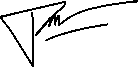
\includegraphics[width=3.0cm,height=1.45cm,keepaspectratio]{picture/signature-tam.png} &

\includegraphics[width=3.0cm,height=1.45cm,keepaspectratio,trim=40bp 10bp 45bp 10bp,clip]{picture/signature-thinh.png} \tabularnewline[0.15cm]
Phí Vương Tường Tâm & Vũ Hưng Thịnh \tabularnewline
\end{tabular}
\end{center}
\chapter*{CÔNG TRÌNH ĐƯỢC HOÀN THÀNH\\TẠI TRƯỜNG ĐẠI HỌC TÔN ĐỨC THẮNG}

Chúng em xin cam đoan đây là công trình nghiên cứu của nhóm, được thực hiện dưới sự hướng dẫn của giảng viên Dung Cẩm Quang. Các nội dung nghiên cứu và kết quả thực nghiệm trình bày trong báo cáo là trung thực. Số liệu do nhóm thực hiện được tổng hợp từ các lượt huấn luyện và đánh giá đã lưu.

Các nhận xét, kết quả và hình ảnh sử dụng từ công trình của tác giả khác đều được trích dẫn và ghi rõ nguồn gốc.

Chúng em chịu trách nhiệm về nội dung báo cáo và những vi phạm tác quyền, bản quyền do nhóm gây ra trong quá trình thực hiện, nếu có. Trường Đại học Tôn Đức Thắng không liên quan đến những vi phạm này.

\begin{flushright}\textit{TP. Hồ Chí Minh, ngày 25 tháng 10 năm 2026}\end{flushright}
\begin{center}
\begin{tabular}{>{\centering\arraybackslash}m{0.46\textwidth}>{\centering\arraybackslash}m{0.46\textwidth}}
\textit{Tác giả 1} & \textit{Tác giả 2} \tabularnewline[0.15cm]
\textit{(Ký tên và ghi rõ họ tên)} & \textit{(Ký tên và ghi rõ họ tên)} \tabularnewline[0.15cm]
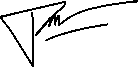
\includegraphics[width=3.0cm,height=1.45cm,keepaspectratio]{picture/signature-tam.png} &

\includegraphics[width=3.0cm,height=1.45cm,keepaspectratio,trim=40bp 10bp 45bp 10bp,clip]{picture/signature-thinh.png} \tabularnewline[0.15cm]
Phí Vương Tường Tâm & Vũ Hưng Thịnh \tabularnewline
\end{tabular}
\end{center}
\chapter*{TÓM TẮT}
Trích xuất thông tin từ hóa đơn đòi hỏi nhận diện đúng ý nghĩa của văn bản trong các bố cục tài liệu khác nhau. Báo cáo khảo sát và so sánh ba hướng tiếp cận thông qua RoBERTa, BROS và PICK, lần lượt sử dụng văn bản; văn bản kết hợp vị trí; và thông tin chữ, ảnh kết hợp đồ thị.

Thực nghiệm được thực hiện trên SROIE, CORD-v2 và WildReceipt, sử dụng văn bản và tọa độ từ chú thích gốc. Các mô hình được đánh giá theo cùng cách chia dữ liệu và cùng phép đo Precision, Recall, F1 ở mức trường--giá trị. Kết quả cho thấy BROS đạt F1 cao nhất trên cả ba bộ dữ liệu trong các cấu hình đã thử nghiệm. RoBERTa cung cấp mốc so sánh chỉ dùng văn bản, trong khi bản triển khai PICK cho kết quả thấp hơn và có những khác biệt so với kiến trúc gốc cần được kiểm chứng thêm.

Kết quả bước đầu cung cấp cơ sở so sánh các phương pháp và phân tích lỗi trích xuất. Phạm vi kết luận giới hạn ở các cấu hình đã chạy; các thí nghiệm mới sử dụng một seed và chưa tách riêng tác động của từng thành phần mô hình.

Từ khóa: trích xuất thông tin, hóa đơn, RoBERTa, BROS, PICK.
\chapter*{ABSTRACT}
Extracting information from receipts requires identifying the meaning of text across varying document layouts. This report compares three approaches through RoBERTa, BROS and PICK, which use text alone, text with spatial information, and a graph-based combination of textual and visual features, respectively.

Experiments are conducted on SROIE, CORD-v2 and WildReceipt using text and bounding boxes from the original annotations. The models are evaluated with shared data splits and a common field--value precision, recall and F1 protocol. BROS achieves the highest F1 on all three datasets among the tested configurations. RoBERTa serves as a text-only baseline, while the implemented PICK variant obtains lower scores and differs from the original architecture in aspects that require further verification.

These preliminary findings support comparison of the methods and analysis of extraction errors. Conclusions are limited to the tested configurations: the experiments use a single random seed and do not isolate the effects of individual model components.

Keywords: information extraction, receipts, RoBERTa, BROS, PICK.
\clearpage
\begingroup
\renewcommand{\baselinestretch}{1.05}\normalsize
\tableofcontents
\endgroup
\clearpage
\phantomsection\addcontentsline{toc}{chapter}{\listfigurename}\listoffigures
\clearpage
\phantomsection\addcontentsline{toc}{chapter}{\listtablename}\listoftables
\chapter*{DANH MỤC CÁC CHỮ VIẾT TẮT}
\addcontentsline{toc}{chapter}{DANH MỤC CÁC CHỮ VIẾT TẮT}
\begin{table}[H]
\centering
\renewcommand{\arraystretch}{1.25}
\fontsize{12}{14}\selectfont
\setlength{\tabcolsep}{4pt}
\begin{tabular}{L{2.4cm}L{12.0cm}}
\toprule
\textbf{Viết tắt} & \textbf{Ý nghĩa} \\
\midrule
KIE & Key Information Extraction -- trích xuất thông tin chính \\
OCR & Optical Character Recognition -- nhận dạng chữ \\
GT & Ground truth -- đáp án tham chiếu \\
BIO & Begin, Inside, Outside -- bắt đầu, bên trong, ngoài thực thể \\
BROS & BERT Relying On Spatiality \\
BiLSTM & Bidirectional Long Short-Term Memory \\
CRF & Conditional Random Field -- trường ngẫu nhiên có điều kiện \\
TP / FP / FN & Đúng / dự đoán thừa hoặc sai / bỏ sót đáp án \\
\bottomrule
\end{tabular}
\end{table}
\clearpage
\pagenumbering{arabic}
